\subsubsection{\textit{Payment service}}
\label{sec:payment-service}

El \textit{payment service} es el encargado de administrar y gestionar la economía del juego. Más adelante se explicará
el modelo económico del juego. El servicio está formado por los siguientes componentes:
\vspace{0.25cm}

\begin{itemize}
  \item \underline{\textit{Gems balance}}: Gestión del estado de los balances de gemas de los jugadores.
  \item \underline{\textit{Gems packs}}: Creación, actualización y eliminación de los paquetes para comprar gemas.
  \item \underline{\textit{Gem Metrics}}: Estado de las gemas compradas y utilizadas en todos los mundos.
  \item \underline{\textit{Creator Balances}}: Estado de las ganancias de los creadores de mundos.
  \item \underline{\textit{Subscriptions}}: Gestión de las suscripciones para activar zonas de mundos.
\end{itemize}

Para acceder a cosméticos, los jugadores deben adquirirlos mediante gemas. Estas se obtienen comprando \textit{packs}, 
y los pagos son gestionados a través de Stripe. Las gemas y los precios de cada \textit{pack} son administrados exclusivamente 
por los administradores del sistema, quienes pueden crear, actualizar y eliminar \textit{packs} mediante los \textit{endpoints} 
correspondientes.
\vspace{0.25cm}

El flujo de compra de gemas comienza cuando el usuario envía una petición a \texttt{POST /payments/} \texttt{checkout},
que crea una sesión de \textit{checkout} de Stripe para el \textit{pack} seleccionado. Una vez que el usuario
completa el pago en la plataforma de Stripe, esta notifica al sistema a través del \textit{endpoint} de
\textit{webhook} \, \texttt{POST /payments/webhook/stripe}, que procesa el evento y acredita las gemas
correspondientes en el balance del usuario. El evento esperado es \texttt{payment\_intent.succeeded}.

\vspace{0.25cm}

\begin{figure}[H]
    \centering
    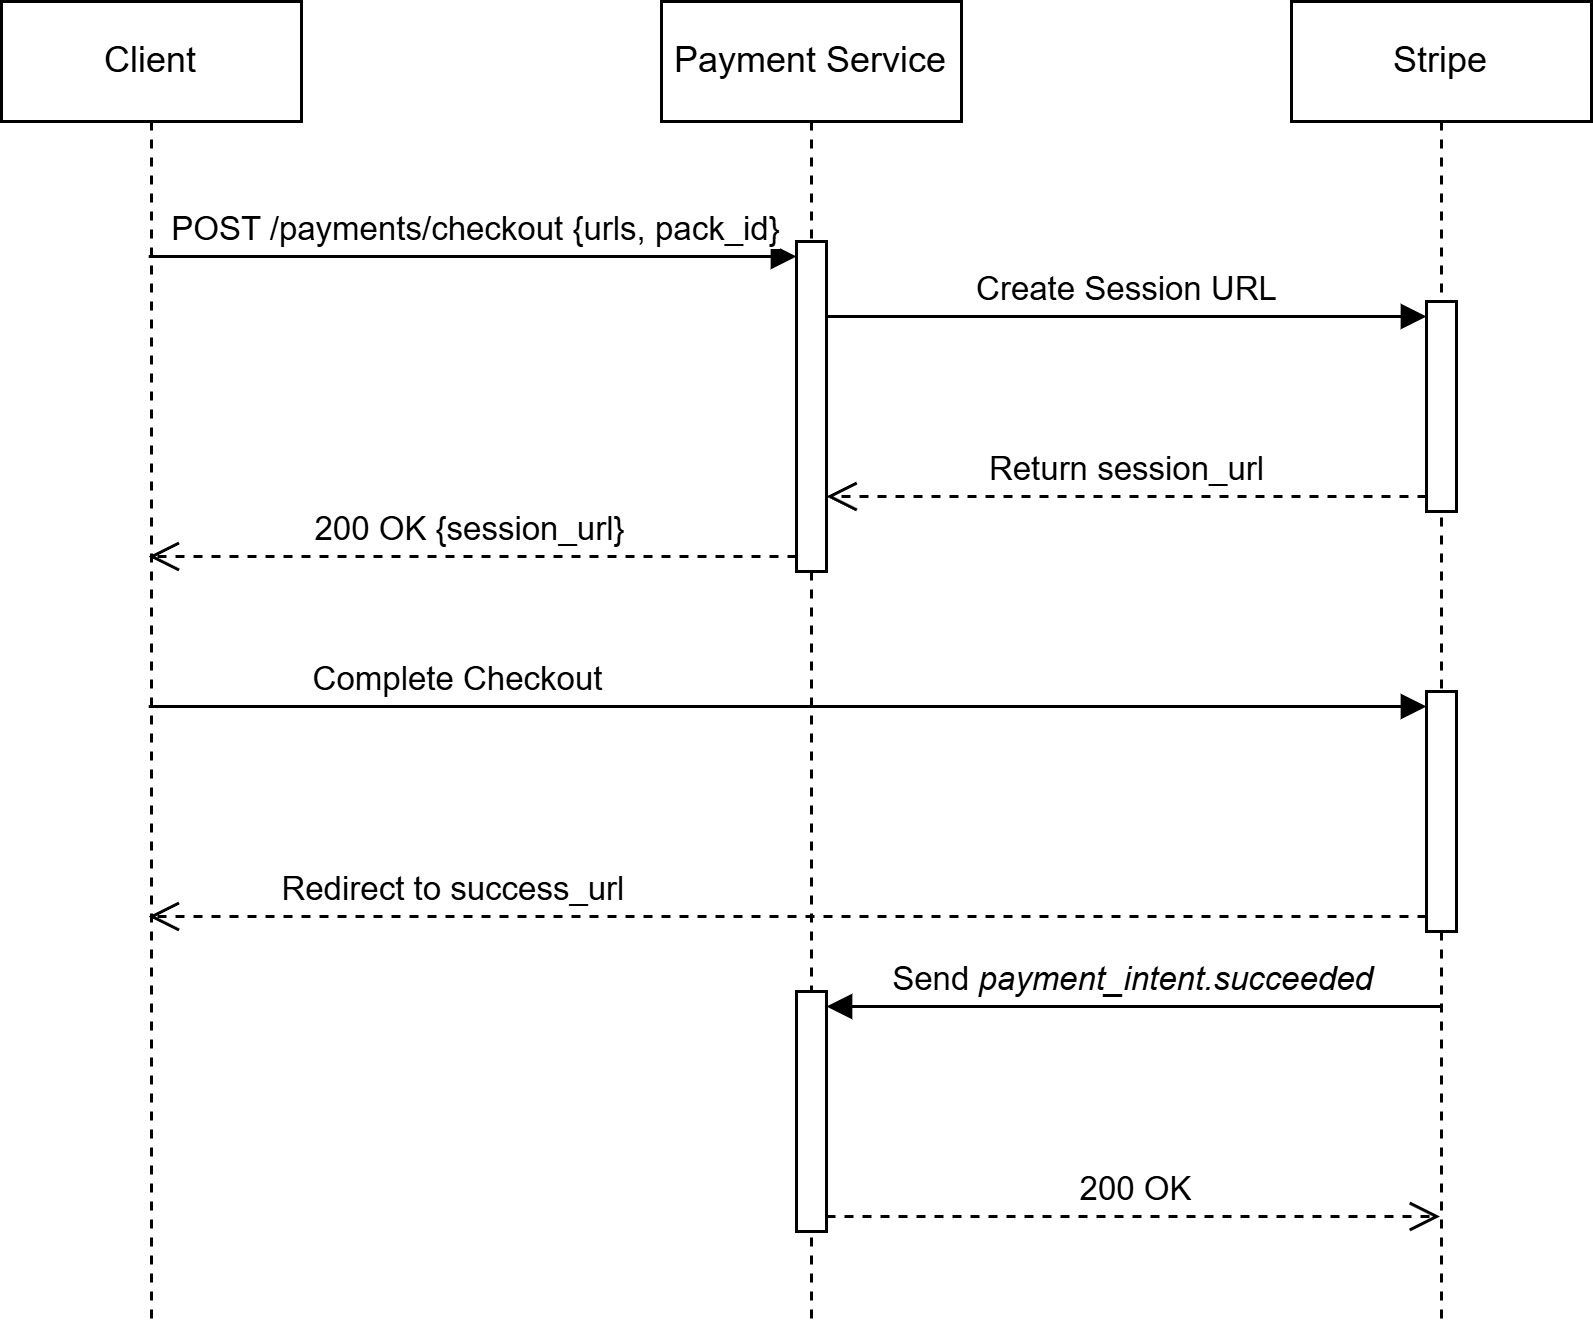
\includegraphics[width=0.75\textwidth]{img/08-implemented-solution/core-service/payment-service-case-1.jpg}
    \caption{Diagrama de secuencia del flujo de compra de gemas}
    \label{fig:payment-service-case-1}
\end{figure}

Una vez completada la transacción, Stripe redirige al usuario a una página de confirmación o error según el resultado del pago.
Para ello, se ejecuta un servidor local en el cliente que gestiona estas páginas de redirección, las cuales se especifican
como parámetros al crear la sesión de \textit{checkout}. Adicionalmente, cuando la compra se procesa correctamente, se envía
automáticamente un correo electrónico al jugador confirmando la transacción y detallando los gemas adquiridas.
\vspace{0.25cm}

El sistema ofrece un mecanismo de suscripción para que los creadores puedan habilitar zonas en sus mundos. La suscripción 
se gestiona por \textit{slots}, donde cada \textit{slot} permite a un creador activar una zona en el mundo. 
El estado de la suscripción activa del usuario puede consultarse, en cualquier momento, mediante 
\texttt{GET /subscriptions/status}.

\vspace{0.25cm}

El flujo de alta de una suscripción comienza con \texttt{POST /subscriptions/checkout}, que crea una sesión de
\textit{checkout} de Stripe para la suscripción. Una vez completado el pago, Stripe notifica al sistema a través
de \texttt{POST /subscriptions/webhook/stripe}, que procesa los eventos de alta, modificación y cancelación de
suscripciones. Similar a las gemas, sin embargo aquí se recibe el evento \texttt{customer.subscription.created}.
\vspace{0.25cm}

\begin{figure}[H]
    \centering
    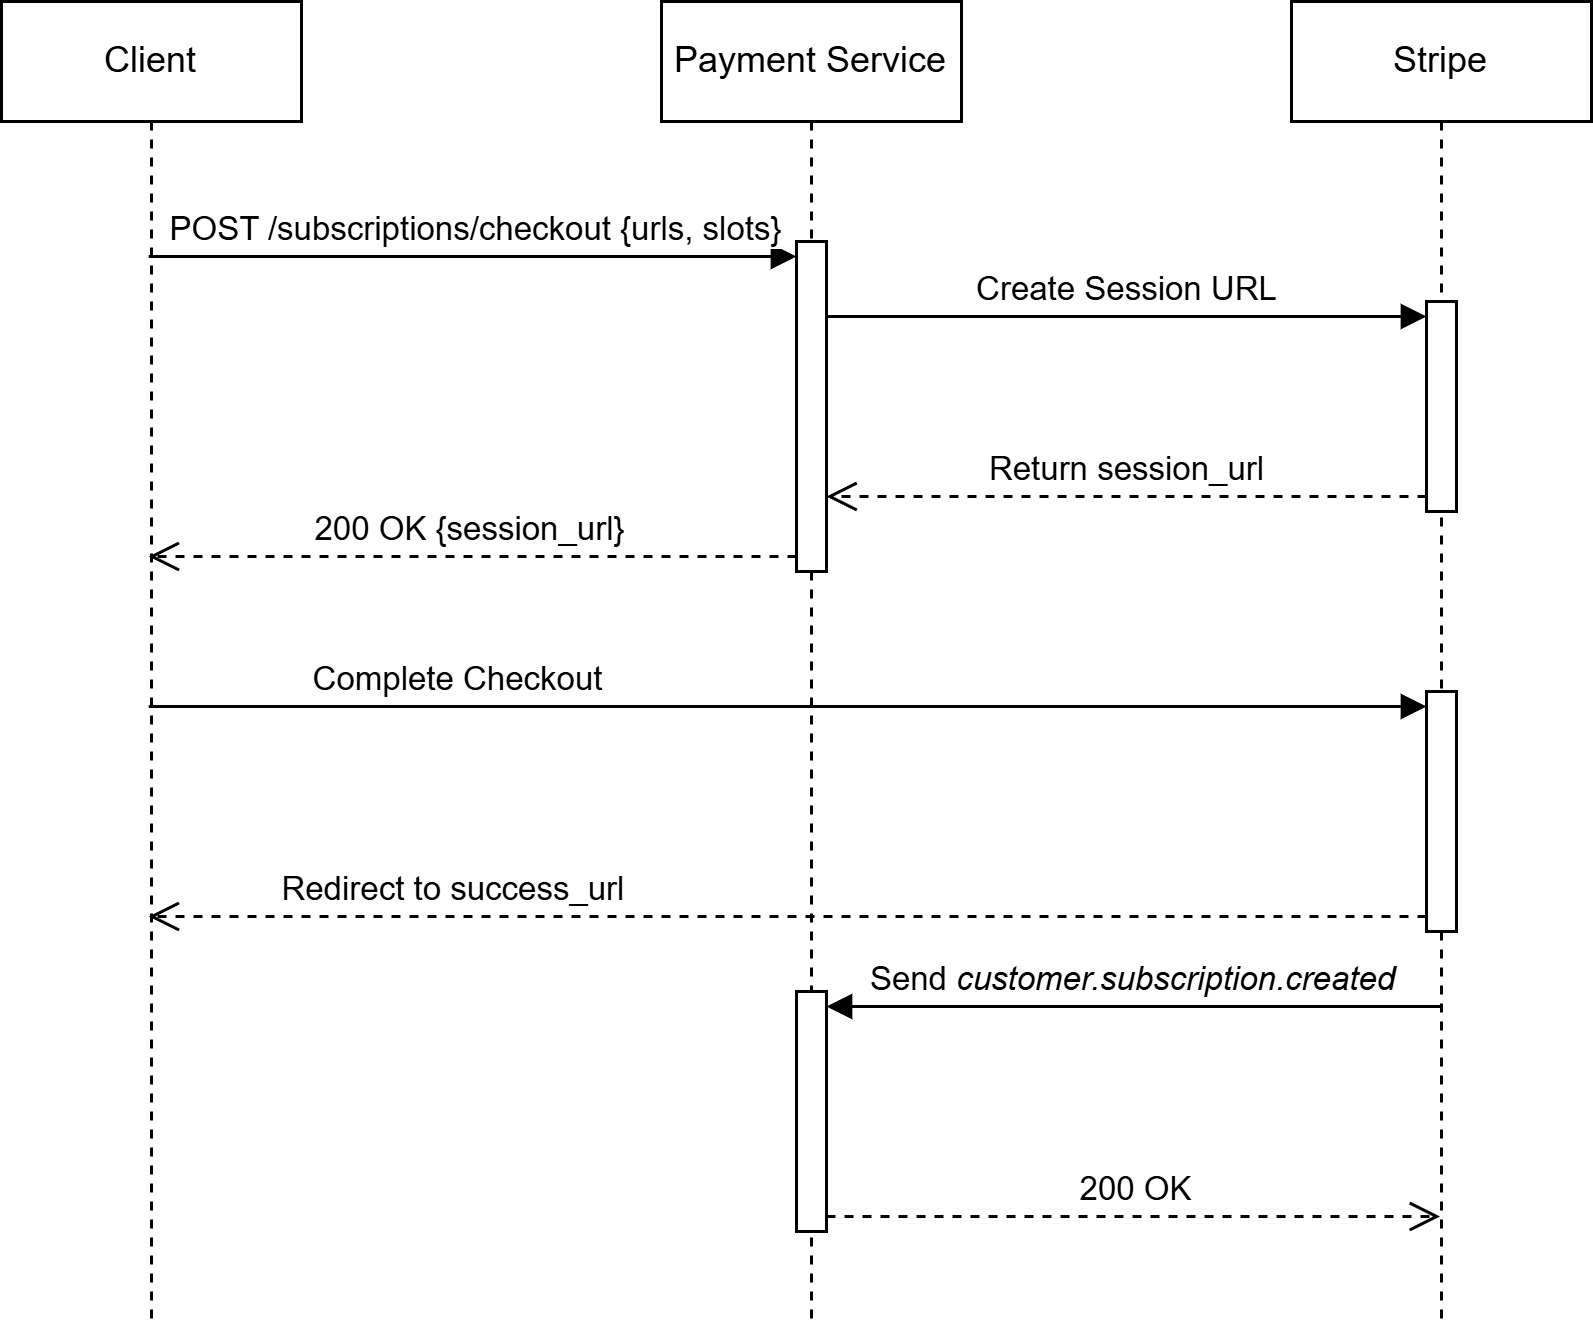
\includegraphics[width=0.75\textwidth]{img/08-implemented-solution/core-service/payment-service-case-2.jpg}
    \caption{Diagrama de secuencia del flujo de subscripcion}
    \label{fig:payment-service-case-2}
\end{figure}

Una vez activa la suscripción, el usuario puede ajustar la cantidad de \textit{slots} contratados mediante
\texttt{PUT /subscriptions/slots} (aplicando los cambios de tarifas correspondientes), y cancelarla mediante 
\texttt{DELETE /subscriptions}, siempre que no tenga \textit{slots} en uso en ese momento. 
Los eventos que se reciben, respectivamente, son \texttt{customer.subscription.updated}
y \texttt{customer.subscription.deleted}.
\vspace{0.25cm}

Por último, el servicio expone dos \textit{endpoints} de uso interno para
la comunicación entre servicios: \texttt{GET /subscriptions/internal/users/\{user\_id\}/} \texttt{status}, que permite
verificar la disponibilidad de \textit{slots} para un usuario, y \texttt{PUT /subscriptions/} \texttt{internal/users/\{user\_id\}} 
\texttt{/used-slots}, que actualiza la cantidad de \textit{slots} consumidos. Todos estos eventos son notificados mediante email.
\vspace{0.25cm}

Cuando un usuario desea adquirir un cosmético, envía una petición a
\texttt{POST /payments/gems/} \texttt{balances/purchase/\{cosmetic\_id\}}. El flujo interno que se desencadena consta de
varios pasos que involucran comunicación entre servicios.
\vspace{0.25cm}

En primer lugar, el \textit{payment service} consulta al \textit{assets service} mediante el \textit{endpoint}
interno \texttt{GET /assets/internal/cosmetics/\{cosmetic\_id\}} para obtener el precio del cosmético y el
identificador de su creador. A continuación, verifica que el balance de gemas del usuario sea suficiente para
cubrir dicho precio; si no lo es, retorna un error indicando gemas insuficientes.
\vspace{0.25cm}

\begin{figure}[H]
    \centering
    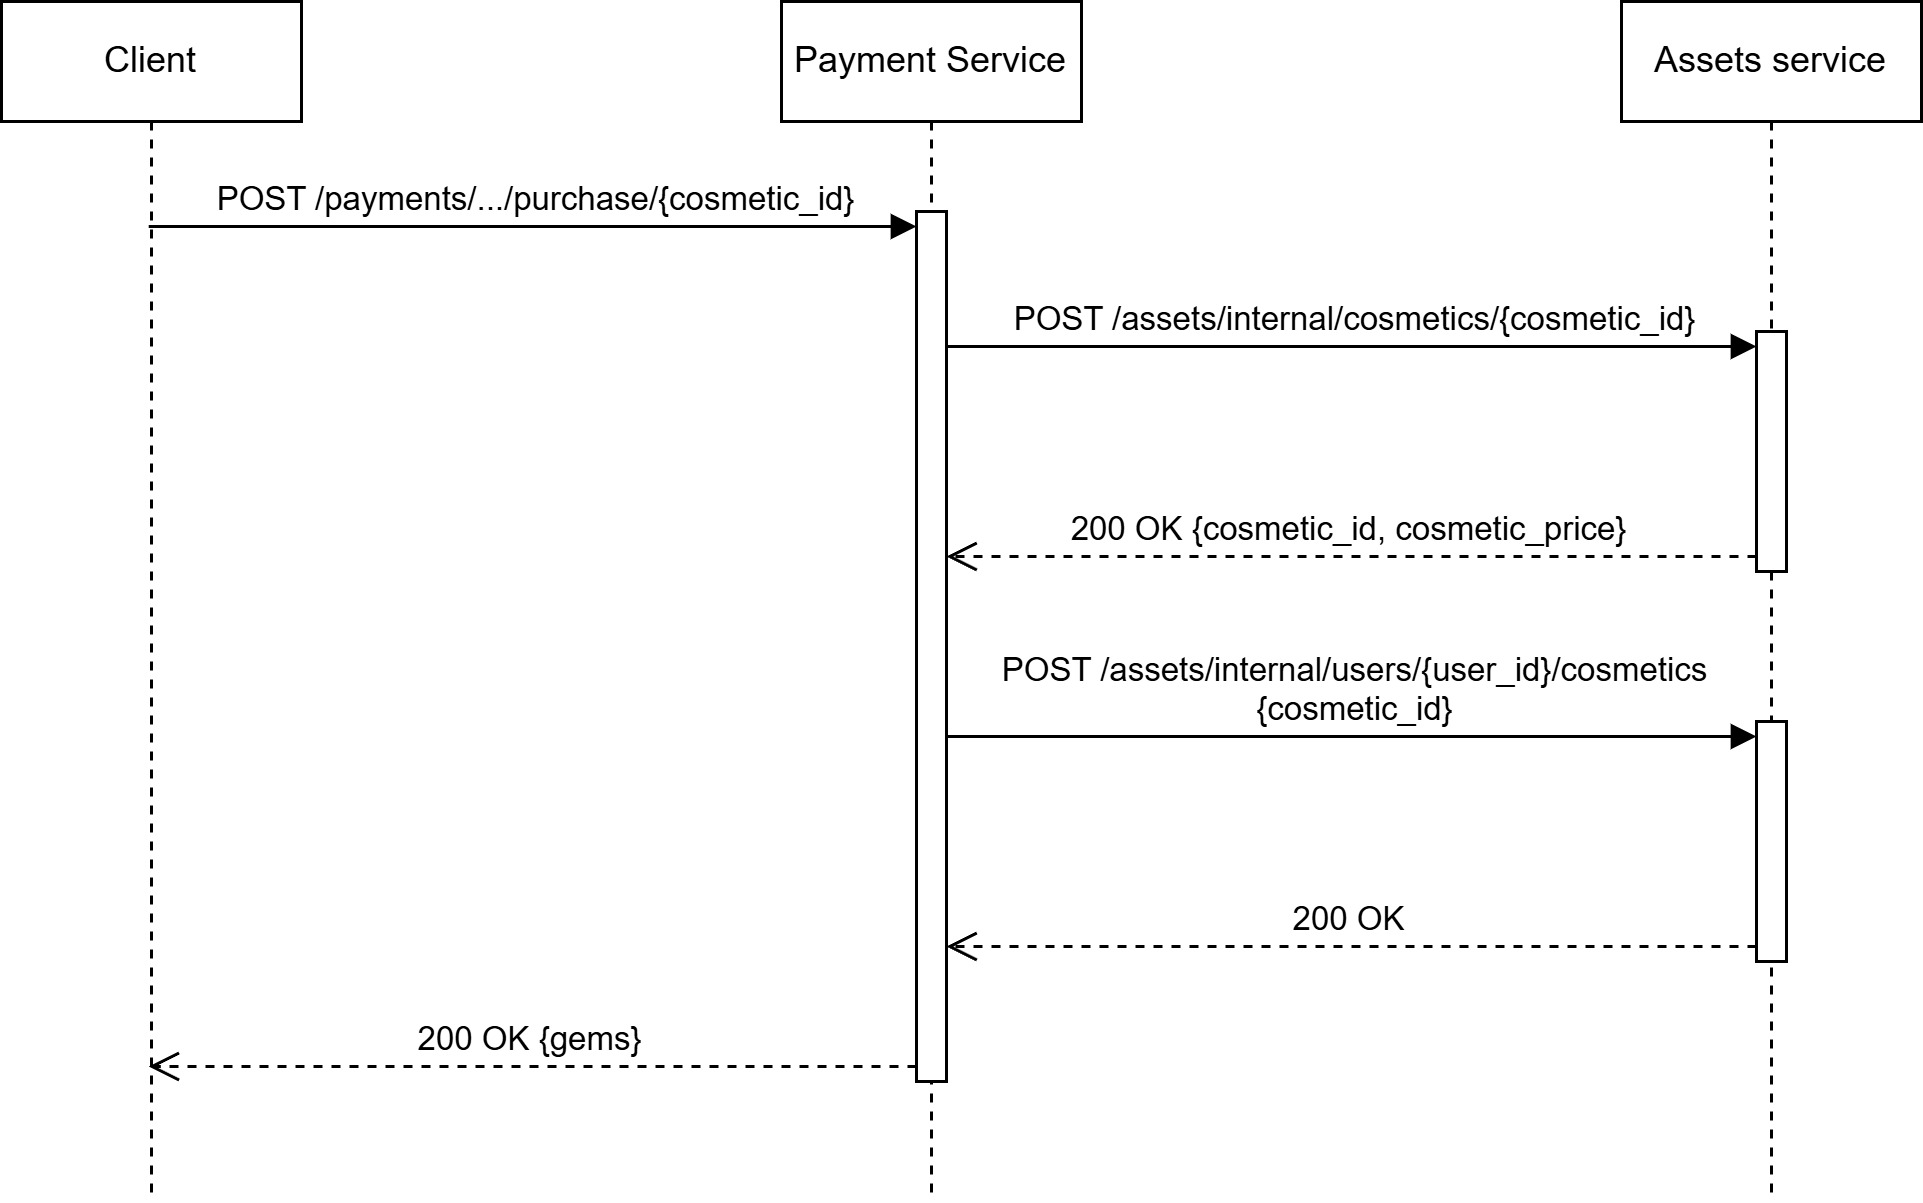
\includegraphics[width=0.95\textwidth]{img/08-implemented-solution/core-service/payment-service-case-3.jpg}
    \caption{Diagrama de secuencia de la compra de un cosmético}
    \label{fig:payment-service-case-3}
\end{figure}

Si el balance es suficiente, se registra la compra en el \textit{assets service} mediante el \textit{endpoint}
interno \texttt{POST /assets/internal/users/\{user\_id\}/cosmetics}. Este paso puede retornar un error de
conflicto si el usuario ya había adquirido el cosmético previamente. Una vez confirmado el registro, se deducen
las gemas del balance del usuario.
\vspace{0.25cm}

Finalmente, si el cosmético tiene un precio mayor a cero y fue creado por un usuario distinto al sistema, se
acredita una porción de las gemas al creador en forma de balance en dólares. El monto se calcula aplicando
el porcentaje de reparto configurado (\texttt{CreatorRevenuePercent}) sobre el precio en gemas, convertido
a dólares mediante la tasa de cambio configurada (\texttt{DollarsGems} \texttt{Ratio}). Este balance se 
acumula a lo largo del tiempo con cada compra. Adicionalmente, se actualizan las métricas globales de 
gemas gastadas en las compras. 

\vspace{0.25cm}

Un creador puede consultar su propio balance en cualquier momento mediante \texttt{GET /payments} \texttt{/balances/creators},
que retorna el monto acumulado. Los administradores disponen adicionalmente del
\textit{endpoint} \, \texttt{GET /payments/balances/creators/all}, que retorna los balances de la totalidad de los
creadores del sistema.
\vspace{0.25cm}

El sistema mantiene métricas agregadas sobre la actividad económica relacionada con las gemas, accesibles
exclusivamente para administradores mediante \texttt{GET /payments/gems/metrics}. Las métricas expuestas son
las gemas compradas en total (\texttt{gems\_bought}), las gemas gastadas en cosméticos (\texttt{gems\_spent}),
los ingresos generados por la venta de gemas (\texttt{gems\_revenue}) y el flujo de gemas (\texttt{gems\_flow}),
que representa la proporción entre las gemas gastadas y las compradas. Este último indicador permite evaluar
qué fracción de las gemas adquiridas está siendo efectivamente utilizada en el sistema.
\vspace{0.25cm}
